
\documentclass[xcolor=dvipsnames]{beamer} 
\usetheme{default} 

\usecolortheme[named=Blue]{structure}
\usetheme[height=7mm]{Rochester} 
\setbeamertemplate{items}[ball] 
\setbeamertemplate{blocks}[rounded]
\setbeamertemplate{navigation symbols}{} 

\usepackage{tikz} 
\usetikzlibrary{shapes.arrows,chains,positioning,decorations.pathreplacing}

% -------------------------------------------------------------------------
% Commands
% -------------------------------------------------------------------------

\newcommand{\addone}[2]{ 
  
  \node (plus1) [inner sep=0pt,draw,circle, fill=blue!50,below= 1em of #1] {\tiny +1};
  \draw (#1) -- (plus1);
  \draw [->] (plus1) -- (#2);   
} 

\newcommand{\sumupPrim}[2]{

  \node (sumup) [inner sep=0pt,draw,circle, fill=blue!50,below= 1em of #1] {\tiny +};
  \draw (#1) -- (sumup);
  \draw [->] (sumup) -- (#2);   
}

\newcommand{\sumup}[2]{

  \node (sumup) [inner sep=0pt,draw,circle, fill=blue!50,below= 1em of #1] {\tiny +};
  \draw (#1) -- (sumup);
  \draw [->] (sumup) |- (#2);   
}

\newcommand{\adder}[3]{ 
  \node (adder) [inner sep=0pt,draw,circle, fill=blue!50,below right= 0.5em and -0.2em of #1] {\tiny +};
  \draw (#1.south) |- (adder); 
  \draw (#2.south) |- (adder); 
  \draw [->] (adder) -- (#3.north);     
} 


\begin{document}

% -------------------------------------------------------------------------
%
% -------------------------------------------------------------------------

\title{Embedded Languages for Data-Parallel Programming} 
\author[J. Svensson]{Bo Joel Svensson} 
\institute{ 
  Department of Computer Science and Engineering \\ 
  Chalmers University of Technology 
} 

% -------------------------------------------------------------------------
%
% -------------------------------------------------------------------------

\begin{frame}[plain] 
  \titlepage
\end{frame} 


\section{background} 

% -------------------------------------------------------------------------
% What is data parallelism ?
%   * Fine grained
%   * Scalable (more data -> more potential for parallelism) 
%   
% -------------------------------------------------------------------------
\begin{frame}{Data-Parallelism: Increment}
\begin{center} 
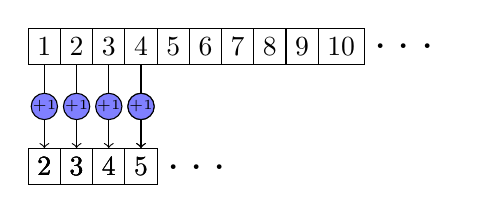
\begin{tikzpicture}[
      start chain=1 going right,start chain=2 going below,node distance=-0.15mm
    ]


  \foreach \x in {1,2,...,10} {
    \node (\x) [draw, on chain=1] {\x};
  }
  \node [on chain=1] {\huge \ldots};
  
  

  \onslide<2>{
    \node [draw, below=3em of 1] (r1) {2};
    % \draw [->] (1) -- (r1);
    \addone{1}{r1}
    }

  \onslide<3>{
    \node [draw, below=3em of 1] (r1) {2};
    \node [draw, below=3em of 2] (r2) {3};
    %\draw [->] (2) -- (r2);
    \addone{2}{r2}
    }


  \onslide<4>{
    \node [draw, below=3em of 1] (r1) {2};
    \node [draw, below=3em of 2] (r2) {3};
    \node [draw, below=3em of 3] (r3) {4};
    %\draw [->] (3) -- (r3);
    \addone{3}{r3}
    }

  \onslide<5>{
    \node [draw, below=3em of 1] (r1) {2};
    \node [draw, below=3em of 2] (r2) {3};
    \node [draw, below=3em of 3] (r3) {4};
    \node [draw, below=3em of 4] (r4) {5};
    %\draw [->] (4) -- (r4);
    \addone{4}{r4}
    }
  
  \onslide<6>{
    \node [draw, below=3em of 1] (r1) {2};
    \node [draw, below=3em of 2] (r2) {3};
    \node [draw, below=3em of 3] (r3) {4};
    \node [draw, below=3em of 4] (r4) {5};
    %\draw [->] (4) -- (r4);
    \addone{4}{r4}
    \node [right=-0.15mm of r4] {\huge \ldots};
    }
  
\end{tikzpicture} 
\end{center}
\end{frame}

% -------------------------------------------------------------------------
%
% -------------------------------------------------------------------------
\begin{frame}{Data-Parallelism: Increment in parallel}
\begin{center} 
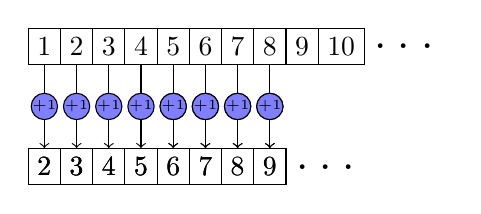
\begin{tikzpicture}[
      start chain=1 going right,start chain=2 going below,node distance=-0.15mm
    ]


  \foreach \x in {1,2,...,10} {
    \node (\x) [draw, on chain=1] {\x};
  }
  \node [on chain=1] {\huge \ldots};
  
  

  \onslide<2>{
    \node [draw, below=3em of 1] (r1) {2};
    \node [draw, below=3em of 2] (r2) {3};
    \node [draw, below=3em of 3] (r3) {4};
    \node [draw, below=3em of 4] (r4) {5};

    \addone{1}{r1}
    \addone{2}{r2}
    \addone{3}{r3}
    \addone{4}{r4}
    %\draw [->] (1) -- (r1);
    %\draw [->] (2) -- (r2);
    %\draw [->] (3) -- (r3);
    %\draw [->] (4) -- (r4);
    }

  \onslide<3>{
    \node [draw, below=3em of 1] (r1) {2};
    \node [draw, below=3em of 2] (r2) {3};
    \node [draw, below=3em of 3] (r3) {4};
    \node [draw, below=3em of 4] (r4) {5};
    \node [draw, below=3em of 5] (r5) {6};
    \node [draw, below=3em of 6] (r6) {7};
    \node [draw, below=3em of 7] (r7) {8};
    \node [draw, below=3em of 8] (r8) {9};

    \addone{5}{r5}
    \addone{6}{r6}
    \addone{7}{r7}
    \addone{8}{r8}
    }

  \onslide<3>{
    \node [draw, below=3em of 1] (r1) {2};
    \node [draw, below=3em of 2] (r2) {3};
    \node [draw, below=3em of 3] (r3) {4};
    \node [draw, below=3em of 4] (r4) {5};
    \node [draw, below=3em of 5] (r5) {6};
    \node [draw, below=3em of 6] (r6) {7};
    \node [draw, below=3em of 7] (r7) {8};
    \node [draw, below=3em of 8] (r8) {9};

    \addone{5}{r5}
    \addone{6}{r6}
    \addone{7}{r7}
    \addone{8}{r8}

    \node [right=-0.15mm of r8] {\huge \ldots};
    }

\end{tikzpicture} 

\end{center}
\end{frame}

% -------------------------------------------------------------------------
% Computing a sum
% -------------------------------------------------------------------------
\begin{frame}{Data-Parallelism: Sum}
\begin{center} 
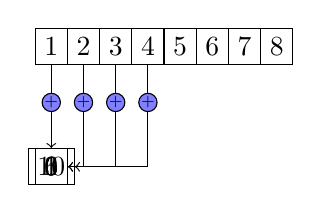
\begin{tikzpicture}[
      start chain=1 going right,start chain=2 going below, node distance=-0.15mm
    ]


  \foreach \x in {1,2,...,8} {
    \node (\x) [draw, on chain=1] {\x};
  }
  % \node [on chain=1] {\huge \ldots};
  
  \onslide<2>{
    \node [draw, below=3em of 1] (r1) {0};
    %\draw [->] (1) -- (r1);
    }

  
  \onslide<3>{
    \node [draw, below=3em of 1] (r1) {1};
    %\draw [->] (1) -- (r1);
    \sumupPrim{1.south}{r1.north}
    }
  
  \onslide<4>{
    \node [draw, below=3em of 1] (r1) {3};
    %\draw [->] (2.south) |- (r1.east);
    \sumup{2.south}{r1.east}
    }
  
  \onslide<5>{
    \node [draw, below=3em of 1] (r1) {6};
    %\draw [->] (3.south) |- (r1.east);
    \sumup{3.south}{r1.east}
    }

  \onslide<6>{
    \node [draw, below=3em of 1] (r1) {10};
    %\draw [->] (4.south) |- (r1.east);
    \sumup{4.south}{r1.east}
    }




\end{tikzpicture} 
\end{center}
\end{frame}

% -------------------------------------------------------------------------
% Computing a sum in parallel 
% -------------------------------------------------------------------------

\begin{frame}{Data-Parallelism: Sum in parallel}
\begin{center} 
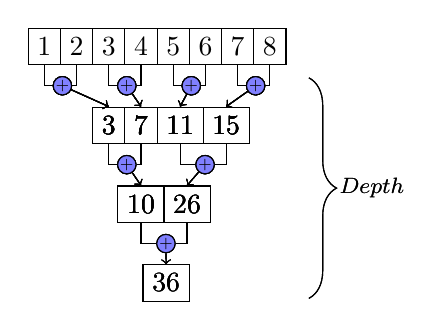
\begin{tikzpicture}[
      start chain=1 going right,start chain=2 going below,node distance=-0.15mm
    ]


  \foreach \x in {1,2,...,8} {
    \node (\x) [draw, on chain=1] {\x};
  }
  
  \onslide<2>{
    \node (imm1) [draw,below=1.5em of 3] {3};
    \node (imm2) [draw,right= of imm1] {7};
    \node (imm3) [draw,right= of imm2] {11};
    \node (imm4) [draw,right= of imm3] {15};
    
    \adder{1}{2}{imm1}
    \adder{3}{4}{imm2}
    \adder{5}{6}{imm3}
    \adder{7}{8}{imm4}
   
  }

  \onslide<3>{
    \node (imm1) [draw,below=1.5em of 3] {3};
    \node (imm2) [draw,right= of imm1] {7};
    \node (imm3) [draw,right= of imm2] {11};
    \node (imm4) [draw,right= of imm3] {15};

    \adder{1}{2}{imm1}
    \adder{3}{4}{imm2}
    \adder{5}{6}{imm3}
    \adder{7}{8}{imm4}
   
    \node (jmm1) [draw,below=1.5em of imm2] {10};
    \node (jmm2) [draw,right= of jmm1] {26};

    \adder{imm1}{imm2}{jmm1}
    \adder{imm3}{imm4}{jmm2} 
  }

 \onslide<4>{
    \node (imm1) [draw,below=1.5em of 3] {3};
    \node (imm2) [draw,right= of imm1] {7};
    \node (imm3) [draw,right= of imm2] {11};
    \node (imm4) [draw,right= of imm3] {15};

    \adder{1}{2}{imm1}
    \adder{3}{4}{imm2}
    \adder{5}{6}{imm3}
    \adder{7}{8}{imm4}

    \node (jmm1) [draw,below=1.5em of imm2] {10};
    \node (jmm2) [draw,right= of jmm1] {26};

    \adder{imm1}{imm2}{jmm1}
    \adder{imm3}{imm4}{jmm2}

    \node (lmm1) [draw,below right=1.5em and -0.8em of jmm1] {36};
    
    \adder{jmm1}{jmm2}{lmm1} 
  }

  \onslide<5>{
    \node (imm1) [draw,below=1.5em of 3] {3};
    \node (imm2) [draw,right= of imm1] {7};
    \node (imm3) [draw,right= of imm2] {11};
    \node (imm4) [draw,right= of imm3] {15};

    \adder{1}{2}{imm1}
    \adder{3}{4}{imm2}
    \adder{5}{6}{imm3}
    \adder{7}{8}{imm4}

    \node (jmm1) [draw,below=1.5em of imm2] {10};
    \node (jmm2) [draw,right= of jmm1] {26};

    \adder{imm1}{imm2}{jmm1}
    \adder{imm3}{imm4}{jmm2}

    \node (lmm1) [draw,below right=1.5em and -0.8em of jmm1] {36};
    
    \adder{jmm1}{jmm2}{lmm1}

    \draw [decorate,
           decoration={brace,mirror,amplitude=10pt},xshift=-4pt,yshift=0pt]
          (3.5,-3.2) -- (3.5,-0.4) node [black,midway,xshift=0.8cm]  
          {\footnotesize $Depth$};
  }

 \onslide<6>{
    \node (imm1) [draw,below=1.5em of 3] {3};
    \node (imm2) [draw,right= of imm1] {7};
    \node (imm3) [draw,right= of imm2] {11};
    \node (imm4) [draw,right= of imm3] {15};

    \adder{1}{2}{imm1}
    \adder{3}{4}{imm2}
    \adder{5}{6}{imm3}
    \adder{7}{8}{imm4}

    \node (jmm1) [draw,below=1.5em of imm2] {10};
    \node (jmm2) [draw,right= of jmm1] {26};

    \adder{imm1}{imm2}{jmm1}
    \adder{imm3}{imm4}{jmm2}

    \node (lmm1) [draw,below right=1.5em and -0.8em of jmm1] {36};
    
    \adder{jmm1}{jmm2}{lmm1}

    \draw [decorate,
           decoration={brace,mirror,amplitude=10pt},xshift=-4pt,yshift=0pt]
          (3.5,-3.2) -- (3.5,-0.4) node [black,midway,xshift=0.8cm]  
          {\footnotesize $Depth$};
         
  }
\end{tikzpicture} 

\onslide<6>{
   \begin{tikzpicture}[overlay,remember picture] 
      
    \node [fill=red!50,single arrow] at (-3.7,3.5) {\tiny Potential for parallelism};
    \node [fill=red!50,single arrow] at (-2.8,2.4) {\tiny Potential for parallelism};
    \end{tikzpicture}
 
}


\end{center}
\end{frame}

% -------------------------------------------------------------------------
%
% -------------------------------------------------------------------------

\begin{frame}{Data-Parallelism}

  \begin{columns} 

  \begin{column}{.48\textwidth}
  \includegraphics[width=\linewidth]{fallout.jpg}

  Rendering

  \vspace{1cm}
  \includegraphics[width=\linewidth]{kiri.jpg}

  Image processing

  \end{column} 
  
  \begin{column}{.48\textwidth} 
  \includegraphics[width=\linewidth]{mmixedsorter.pdf}

  Sorting

  \end{column}
  
  \end{columns}

\end{frame}


\begin{frame}{Data-Parallelism}

  \begin{itemize} 
    \item Scalable
      \begin{itemize} 
        \item Potential for parallelism increase with data size 
      \end{itemize}
    \item Fine grained parallelism 
  \end{itemize} 

\end{frame}

% -------------------------------------------------------------------------
%
% -------------------------------------------------------------------------
\section{GPUs and CUDA}

\begin{frame}{GPUs} 

\includegraphics[width=\linewidth]{GPU1.pdf}


\end{frame} 

\begin{frame}{GPUs} 

\includegraphics[width=\linewidth]{GPU2.pdf}


\end{frame} 


% -------------------------------------------------------------------------
%
% -------------------------------------------------------------------------


\begin{frame}{GPU Programming}
\begin{center} 

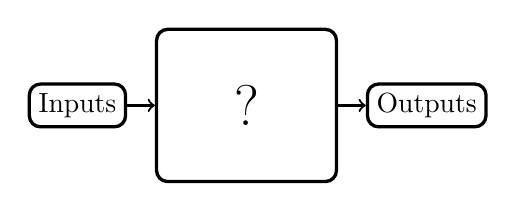
\begin{tikzpicture}[
      start chain=1 going right,start chain=2 going below,node distance=1em,
      every join/.style={->,thick},
    ]

  \node [draw,very thick, rounded corners, on chain=1,join] {Inputs}; 
  \node [draw,very thick, rounded corners, on chain=1,minimum height=5.5em,minimum width = 6.5em,join] {\huge ?}; 
  \node [draw,very thick, rounded corners, on chain=1,join] {Outputs}; 
  

\end{tikzpicture} 
\end{center}

\end{frame}

% -------------------------------------------------------------------------
%
% -------------------------------------------------------------------------
\section{GPUs and CUDA}

\begin{frame}{GPU Programming}
\begin{center} 

\begin{tikzpicture}[remember picture,
      start chain=going right,
      outer/.style={on chain, node distance=1em},
      every join/.style={->,thick},
      inner/.style={circle,draw=blue!50,fill=blue!20,thick,inner sep=1pt},
    ]

  \node [outer,draw,very thick, rounded corners,join] {Inputs}; 
  \node [outer,draw=gray!50,very thick, rounded corners,minimum height=5.5em,minimum width = 6.5em,join] (apa) {
    \begin{tikzpicture} 
      \node [draw=black!100,inner,minimum size=1pt] (k1) {k1};
      \node [draw=black!100,inner,minimum size=1pt, below= 1em of k1] (k2) {k2};
      \node [draw=black!100,inner,minimum size=1pt, right= 1em of k1] (k3) {k3}; 
    \end{tikzpicture}

  }; 
  \node [outer,draw,very thick, rounded corners,join] {Outputs}; 
  

  \draw (k1) -- (k3)
        (k2) -- (k3)
        (apa.west) -- (k1.west)
        (apa.west) -- (k2.west) 
        (k3.east) -- (apa.east); 
  

\end{tikzpicture} 
\end{center}

\end{frame}


% -------------------------------------------------------------------------
%
% -------------------------------------------------------------------------
\section{Embedded Languages}

\begin{frame}{Embedded Languages} 
  
  TODO: 
  \begin{itemize} 
    \item Background, Lava, Compiling embedded languages 
    \item picture: embedded language vs standalone (same as lecture) 
    \item How Bj\"orn and Benny does embedded languages 
  \end{itemize}
  
\end{frame} 

% -------------------------------------------------------------------------
%
% -------------------------------------------------------------------------
\section{Obsidian}
\begin{frame}{Obsidian} 
  
  \begin{itemize} 
    \item our level of GPU programming 
    \item Programming example  (reduction) 
    \item performance 
    \item compare to related approaches 
  \end{itemize}
      
\end{frame} 

% -------------------------------------------------------------------------
%
% -------------------------------------------------------------------------
\section{EmbArBB} 

\begin{frame}{EmbArBB} 
  Embedding ArBB, similar slides to Obsidian, more pictures. 

\end{frame} 



% -------------------------------------------------------------------------
%
% -------------------------------------------------------------------------
\section{Future Work}
\begin{frame}{Future work} 

\end{frame} 


\end{document} 
